\documentclass[11pt,aspectratio=43,ignorenonframetext,t]{beamer}
% Uses fontspec - assumes compiled with LuaLaTeX or similar
% The above \documentclass is for making slides. If making handouts use:
%\documentclass[11pt,a4paper]{article} 
%\usepackage{beamerarticle}
%\setjobnamebeamerversion{main.beamer}

% See https://github.com/CASSON-LAB/uom_beamer_template
% for details on license, further useage information and similar
%%%%%%%%%%%%%%%%%% DOCUMENT SETUP %%%%%%%%%%%%%%%%%%

% Presentation settings
\mode<presentation>{
  \usetheme[framenumber,titleframestart=1]{UoM_alex}
  \usefonttheme{professionalfonts} % using non standard fonts for beamer
  \usefonttheme{serif}             % set font to Arial
  \usepackage{fontspec}
  \setmainfont[Ligatures=TeX]{Arial}
}

% Handout settings
\mode<article>{
  \usepackage{fullpage}                  % use full page
  \usepackage{fontspec}                  % set font to Arial
    \setmainfont[Ligatures=TeX]{Arial}
  \setlength{\parskip}{1.5\baselineskip} % correct beamer line spacings
  \setlength{\parindent}{0cm}
  \usepackage{enumitem}
    \setlist[itemize]{topsep=0pt}
  \definecolor{uomlinkblue}{HTML}{0071BC}
}


% Packages

% Configurando layout para mostrar codigos C++
\usepackage{listings}
\lstset{
  language=HTML,
  basicstyle=\ttfamily\small, 
  keywordstyle=\color{blue}, 
  stringstyle=\color{red}, 
  commentstyle=\color{red}, 
  extendedchars=true, 
  showspaces=false, 
  showstringspaces=false, 
  numbers=left,
  numberstyle=\tiny,
  breaklines=true, 
  backgroundcolor=\color{green!10},
  breakautoindent=true, 
  captionpos=b,
  xleftmargin=0pt,
}

\usepackage{graphicx}  % for graphics files
  \graphicspath{ {./fig/aula4} }
\usepackage{amsmath}   % assumes amsmath package installed
  \allowdisplaybreaks[1] % allow eqnarrays to break across pages
\usepackage{amssymb}   % assumes amsmath package installed 
\usepackage{hyperref} % add hyperlinks to document. Settings are for accessiblity
  \hypersetup{
    colorlinks=true,
    linkcolor=uomlinkblue,
    filecolor=uomlinkblue,      
    urlcolor=uomlinkblue,
	pdflang={en-GB},
}
\usepackage[document]{ragged2e} % left aligned text for accessibility
% experimental - does fundamentally work, if with quite a bit of effort
%\usepackage{axessibility} % LaTeX readable equations for accessibility
%  \tagpdfsetup{tabsorder=structure,uncompress,activate-all,interwordspace=true}
%  \pdfextension catalog{/Lang (en-GB)}
%  \RequirePackage{luacode}
%  \directlua{require("axessibility.lua")}
\usepackage{unicode-math} % unicode maths for accessibility
\usepackage{pdfcomment} % for alt text for accessibility
\usepackage{rotating}  % allow portrait figures and tables
\usepackage{subfigure} % allow matrices of figures
\usepackage{float}     % allows H option on floats to force here placement
\usepackage{multirow}  % allows merging of rows in tables
\usepackage{tabularx}  % allows fixed width tables
\usepackage{ctable}    % modifies \hline for use in table
\usepackage{bm}        % allow bold fonts in equations
\usepackage{pgf}       % allow graphics manipulation
\usepackage{media9}    % allow interactive flash files to be embedded
  \addmediapath{../media}
\usepackage{etoolbox}
  \makeatletter \preto{\@verbatim}{\topsep=0pt \partopsep=0pt} \makeatother  
  
% Custom commands
\newcommand{\matlab}{\emph{\sc{Matlab}}}
\newcommand{\maple}{\emph{\sc{Maple}}}
\newcommand{\simulink}{\emph{\sc{Simulink}}}
\newcommand{\dc}{d.c.}
\newcommand{\ac}{a.c.}
\newcommand{\rms}{RMS}
\newcommand{\wgn}{{\tt wgn}}
\newcommand{\sus}[1]{$^{\mbox{\scriptsize #1}}$}
\newcommand{\sub}[1]{$_{\mbox{\scriptsize #1}}$}
\newcommand{\chap}[1]{Chapter~\ref{#1}}
\newcommand{\sect}[1]{Section~\ref{#1}}
\newcommand{\fig}[1]{Fig.~\ref{#1}}
\newcommand{\tab}[1]{Table~\ref{#1}}
\newcommand{\equ}[1]{(\ref{#1})}
\newcommand{\appx}[1]{Appendix~\ref{#1}}
\newcommand{\degree}{\ensuremath{^\circ}}
\newcommand{\Vrms}{Vrms}
\newcommand{\Vpp}{V\sub{pp}}
\newcommand{\otoprule}{\midrule[\heavyrulewidth]}         
\newcolumntype{Z}{>{\centering\arraybackslash}X}  % tabularx centered columns 
\makeatletter \DeclareRobustCommand{\em}{\@nomath\em \if b\expandafter\@car\f@series\@nil \normalfont \else \bfseries \fi} \makeatother
\newcounter{example_number} % keep track of the example questions



%%%%%%%%%%%%%%%%%% FRONT MATTER %%%%%%%%%%%%%%%%%%
\title{Análise Orientada a objetos}
\subtitle{Aula 4}
\author{Prof. Me. Juliana Costa-Silva}
\begin{document}
%%%%%%%%%%%%%%%%%% TITLE SLIDE %%%%%%%%%%%%%%%%%%
\mode<presentation>{ \frame{\titlepage \label{slide:a}}} 
%\begin{figure}[!ht] 
%\fbox{\includeslide[width=\textwidth]{slide:a}} \end{figure}



%%%%%%%%%%%%%%%%%% NEW SLIDE %%%%%%%%%%%%%%%%%%
\clearpage 
\mode<presentation>{\begin{frame}{Na aula de hoje...}
  \setbeamertemplate{section in toc}[sections numbered]
  \tableofcontents[hideallsubsections]
\end{frame}}
%----------------------------------------------------------------------------
\section{Entrada de Dados}
\mode<presentation>{\begin{frame}{Entrada de dados}
  A leitura do console (teclado) obtém dados a partir do objeto   
\textit{System.in}.
  \begin{itemize}
    \item Objetos System.in leem somente bytes;
    \item Por isso é necessário transforma-lo em um objeto 
   \textit{InputStreamReader}.
 \item O \textit{InputStreamReader} lê somente caracteres, então criamos 
um \textit{BufferedReader}.
   \item O \textit{BufferedReader} é um objeto que acopla vários 
caracteres lidos (uma frase por exemplo).
  \end{itemize}
\end{frame}}
%----------------------------------------------------------------------------
\mode<presentation>{\begin{frame}{Utilizando \textit{BufferedReader}}
   Criando um objeto \textit{BufferedReader}
\small{\lstinputlisting[linerange={9-11}]{
./cod/Aula7Leitura.java } }
Declaração da String que receberá a leitura:
\small{\lstinputlisting[linerange={12-13}]{
./cod/Aula7Leitura.java } }\
\end{frame}}
%----------------------------------------------------------------------------
\mode<presentation>{\begin{frame}{Utilizando \textit{BufferedReader}}
  Executando a leitura:
\small{\lstinputlisting[linerange={14-20}]{
./cod/Aula7Leitura.java } }
Para saber sobre as diferenças da classe Scanner leia:\\
\href{https://www.devmedia.com.br/entrada-de-dados-classe-scanner/21366}[
https://www.devmedia.com.br/entrada-de-dados-classe-scanner/21366]
\end{frame}}
%--------------------------------------------e--------------------------------
\section{Introdução a POO}
\mode<presentation>{\begin{frame}{Paradigmas de Programação}
  \begin{itemize}
   \item \textbf{Definição:} Conjunto de regras e/ou hipóteses que governam a 
definição de um modelo.
     \item \textbf{Aplicação:} Auxilia na conduta do processo de busca da 
solução (modelo conceitual) de um problema.
  \end{itemize}
  
\textbf{Paradigmas de Programação:}\\
Estruturado e Orientado a Objetos.
\end{frame}}
%----------------------------------------------------------------------------
\mode<presentation>{\begin{frame}{Paradigmas de Programação}{Estruturado}
  \begin{itemize}
   \item \textbf{Estruturado:} Enfase em processos. Trabalha com a 
identificação de processos, que são aplicados sequencialmente sobre dados para 
realizar a computação desejada (foco nas ações, procedimentos e funções).
     \item Muitas variáveis/ muitas funções/ manutenção difícil
  \end{itemize}
\begin{center}
    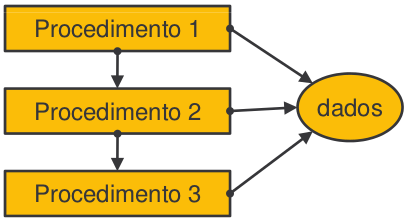
\includegraphics[height=0.25\paperheight]{estruturado.png} \\
  \end{center}
\end{frame}}
%----------------------------------------------------------------------------
\mode<presentation>{\begin{frame}{Paradigmas de Programação}{Orientado a objetos}
  \begin{itemize}
   \item \textbf{Orientado a objetos:} Enfase em dados. Trabalha com entidades 
comportamentais (estado e ações) independentes.
     \item Objeto é a unidade.
     \item Une dados e funções.
  \end{itemize}
\begin{center}
    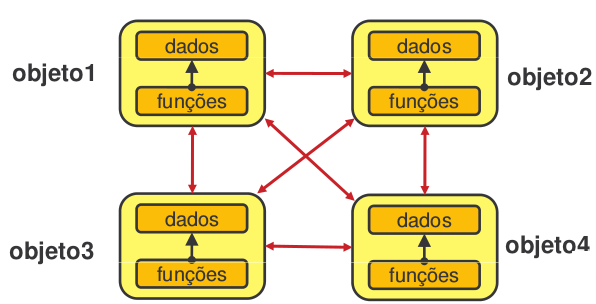
\includegraphics[height=0.35\paperheight]{objetos.png} \\
  \end{center}
\end{frame}}
%----------------------------------------------------------------------------
\mode<presentation>{\begin{frame}{Orientação a objetos}{Introdução}
  Orientação a objetos é uma maneira de programar. Ajuda a organizar o código e 
resolve muitos problemas.

\begin{block}{POO - Definição:}
  \begin{itemize}
   \item ``... um termo geral que inclui qualquer estilo de desenvolvimento que 
seja baseado no conceito de \textbf{\textcolor{red}{objetos}} - uma entidade 
que exibe características e comportamento \cite{sintes2002aprenda}''
     \item ``... uma maneira natural de pensar e escrever programas de 
computador \cite{deitel2010java}''.

  \end{itemize}
\end{block}

\end{frame}}

%----------------------------------------------------------------------------
\mode<presentation>{\begin{frame}{Orientação a Objetos}{Por que mudar o Paradigma?}
\begin{itemize}
  \item ''\textbf{\textcolor{red}{O ser humano conhece o mundo e gerencia sua 
complexidade através de objetos}}. É como desenvolvemos nossa cognição``.
 \item \textbf{Teste:} Explique como funciona a administração de uma 
folha de pagamentos.
 \item E o programa em C para gerenciar isso? Como funcionaria?
 \item No mundo real, funcionário é funcionário.
 \item No aplicativo (C) um funcionário é RecFunc, que realiza tarefas 
implementadas nas funções \textit{CalcSal, IRRFSal}, que estão codificadas nos 
programas Módulo1 e MóduloControle...
\end{itemize}
\end{frame}}
%----------------------------------------------------------------------------
\mode<presentation>{\begin{frame}{Orientação a objetos}
  \begin{itemize}
   \item Na \textbf{Orientação a objetos}, não há separação dos dados e funções.
     \item Objeto é a unidade que une dados e funções.
  \end{itemize}
\begin{center}
    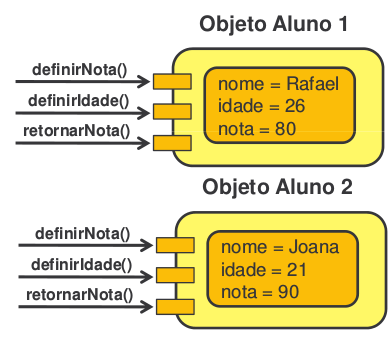
\includegraphics[height=0.5\paperheight]{objAluno.png} \\
  \end{center}
\end{frame}}
%------------------------------------------------------------------
\mode<presentation>{\begin{frame}{Exemplo}
  \begin{columns}
    \begin{column}{0.4\textwidth}
      Estruturado
      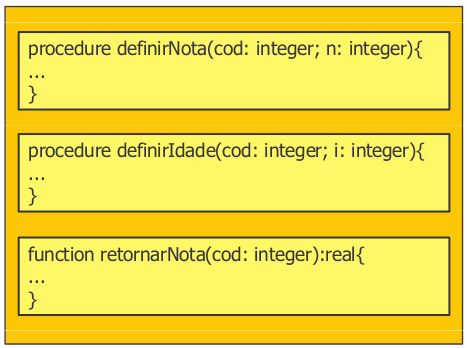
\includegraphics[height=0.4\paperheight]{estAluno.png} \\    
    \end{column}
    
    \begin{column}{0.4\textwidth}
      Orientado a Objetos
     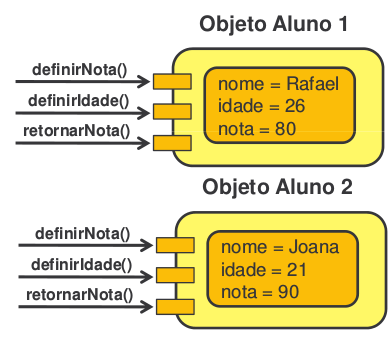
\includegraphics[height=0.4\paperheight]{objAluno.png} \\
    \end{column}

  \end{columns}

\end{frame}}
%---------------------------------------------------------------------
\mode<presentation>{\begin{frame}{\textit{Gap} semântico}
 \begin{itemize}
  \item Diferença entre escopo dos problemas e das soluções
 \end{itemize}
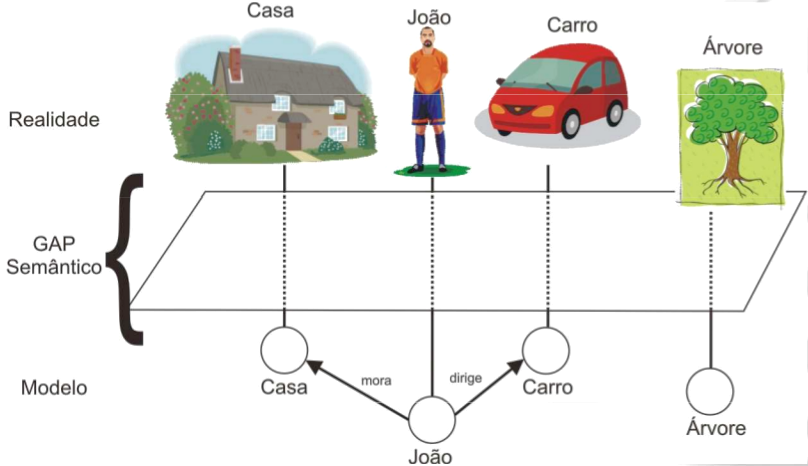
\includegraphics[height=0.6\paperheight]{gapSemantico.png} \\
\end{frame}}

%---------------------------------------------------------------------
\mode<presentation>{\section{Objetos}
\begin{frame}{Objetos}
 \begin{itemize}
  \item Um objeto representa qualquer coisa do mundo real
 \end{itemize}
 \begin{center}
 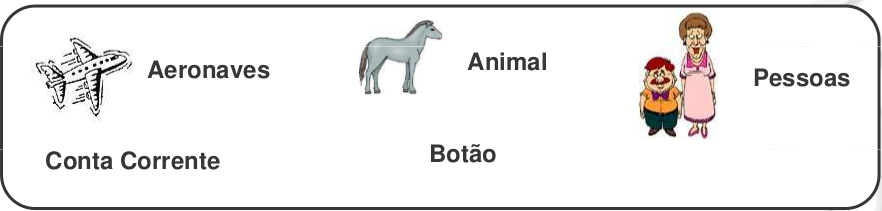
\includegraphics[height=0.2\paperheight]{objetosEx.png}  
 \end{center}
 
 \begin{itemize}
   \item Como no mundo real, os objetos possuem 
\textbf{\textcolor{red}{estado}} e \textbf{\textcolor{red}{comportamento}}.
 \end{itemize}
 \begin{center}
 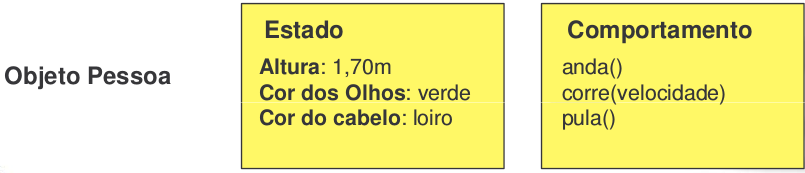
\includegraphics[height=0.2\paperheight]{objPessoa.png}  
 \end{center}
\end{frame}}
%---------------------------------------------------------------------
\mode<presentation>{\begin{frame}{Objeto}
\begin{itemize}
   \item Como no mundo real, os objetos possuem 
\textbf{\textcolor{red}{estado}} e \textbf{\textcolor{red}{comportamento}}.
  \begin{itemize}
    \item \textbf{Estado:} são informações sobre o objeto, como sua cor, 
tamanho, saldo, etc
   \item \textbf{Comportamento:} são ações que o objeto pode realizar, 
como, depositar em uma conta, mudar a cor.
  \end{itemize}
 \end{itemize}
 
 \begin{block}{Quem define o que?}
  \begin{itemize}
   \item Os \textbf{\textcolor{red}{atributos}} definem o \textbf{estado} do 
objeto: \textit{tamanho, cor altura, etc}.
   \item Os \textbf{\textcolor{red}{métodos}} definem o 
\textbf{comportamento} do objeto: \textit{andar, correr, depositar, etc}.
  \end{itemize}
 \end{block}

 \end{frame}}
 %---------------------------------------------------------------------
\mode<presentation>{\begin{frame}{Objetos}
  \begin{block}{Atributos}
   Atributos são similares a variáveis:\\
    \begin{center}
      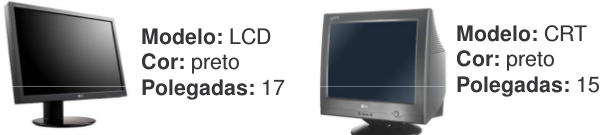
\includegraphics[height=0.15\paperheight]{atributos.png}  
    \end{center}
  \end{block}
  
  \begin{block}{Métodos}
   Métodos são similares a sub rotinas, procedimentos ou funções:\\
    \begin{center}
      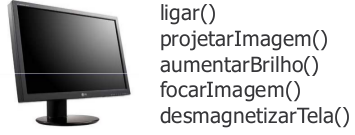
\includegraphics[height=0.15\paperheight]{metodos.png}  
    \end{center}
  \end{block}

\end{frame}}
%---------------------------------------------------------------------
\mode<presentation>{\begin{frame}{Objetos - Visibilidade}
 \begin{itemize}
  \item Como regra geral, os \textbf{\textcolor{red}{atributos}} do objeto 
deverão ser ''\textbf{\textcolor{red}{privados}}`` e somente os 
\textbf{\textcolor{red}{métodos}} do objeto poderão ter acesso a eles. Por que?
   \item Imagine que você está comprando um produto pela internet. Se 
você tivesse a oportunidade de alterar o preço do produto, você não se sentiria 
tentado a faze-lo?
   \item O atributo preço, do objeto produto deve ser modificado somente 
por objetos (ou pessoas) autorizados.
 \end{itemize}
 \begin{center}
  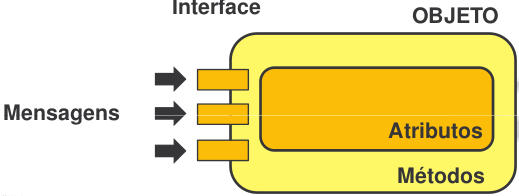
\includegraphics[height=0.2\paperheight]{objInterface.png}
 \end{center}
\end{frame}}
%-------------------------------------------------------------------------
\mode<presentation>{\section{Classes}
\begin{frame}{De onde vem um objeto?}
 \begin{center}
   
\includegraphics[height=0.7\paperheight]{duvidas.jpg} \\
 \end{center}
\end{frame}}
%---------------------------------------------------------------------
\mode<presentation>{\begin{frame}{Classe}
 \begin{itemize}
  \item Modelo ou forma pela qual um objeto é criado
   \item Abstração de um conjunto de objetos que possuem os mesmos tipos 
de características (atributos) e comportamentos (métodos).
   \item Objetos se comportam de acordo com o comportamento da classe que 
os moldou.
 \end{itemize}
  
 \begin{center}
   Classe: Veículo\\
  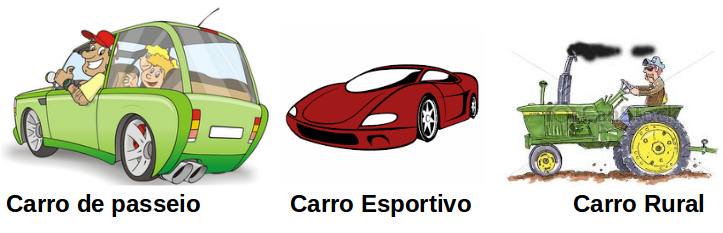
\includegraphics[height=0.25\paperheight]{classeVeiculo.png}\\
  \textbf{Atributos:} cor, passageiros, portas, etc.\\
  \textbf{Métodos:} ligar, desligar, acelerar, parar, etc.
 \end{center}
\end{frame}}
%---------------------------------------------------------------------
\mode<presentation>{\begin{frame}{Conta.java}
  Criando uma classe
\small{\lstinputlisting[linerange={1-8}]{./cod/Conta.java}}
\end{frame}}
%---------------------------------------------------------------------
\mode<presentation>{\begin{frame}{TestaConta.java}
  Declarar e instanciar objeto de uma classe
\small{\lstinputlisting[linerange={1-4}]{./cod/TestaConta.java}}
* Não esqueça de fechar as chaves!!
\end{frame}}
%---------------------------------------------------------------------
\mode<presentation>{\begin{frame}{TestaConta.java}
  Editar objeto de uma classe
\small{\lstinputlisting[linerange={6-8}]{./cod/TestaConta.java}}
\end{frame}}
%---------------------------------------------------------------------
\mode<presentation>{\begin{frame}{TestaConta.java}
  Utilizar objeto de uma classe
\small{\lstinputlisting[linerange={10-10}]{./cod/TestaConta.java}}
\end{frame}}
%---------------------------------------------------------------------
\mode<presentation>{\section{Métodos}
\begin{frame}{Conta.java}
  Método para sacar determinada quantidade de uma conta.
\small{\lstinputlisting[linerange={8-11}]{./cod/Conta.java}}

A expressão \textbf{void} antes do nome do método, indica que o método 
''sacar`` não retorna nenhuma informação.\\
 A variável \underline{novoSaldo }''morre`` no fim do método, assim como 
o argumento \underline{quantidade}. Este é o escopo dessas variáveis.
\end{frame}}
%---------------------------------------------------------------------
\mode<presentation>{\begin{frame}{Métodos com retorno}
  Método que realiza saque de uma conta, somente se houver saldo.
\small{\lstinputlisting[linerange={13-21}]{./cod/Conta.java}}

A expressão \textbf{boolean} antes do nome do método, indica que o método 
''sacarVerifica`` retorna uma informação do tipo boolean.\\
\end{frame}}
%----------------------------------------------------------------------
\mode<presentation>{\section{Atividade}
\begin{frame}{Atividade de Aula}
  \begin{enumerate}
   \item Implemente o método depositar, na classe conta.
   \item Lembre-se que ele deve atualizar o saldo do cliente;
   \item Teste o método criado.
   \item Envie o código desenvolvido em aula, como atividade de aula.
  \end{enumerate}
\end{frame}}
%------------------------------
\section{Leitura recomendada}
\mode<presentation>{\begin{frame}{Leitura complementar}
 Para mais informações sobre JAVA, leia:\\
	\begin{columns}
	\begin{column}{0.5\textwidth}
	 Capítulo 3 a 7:\\
	 \cite{deitel2017java}
	\end{column}
	\begin{column}{0.4\textwidth}
	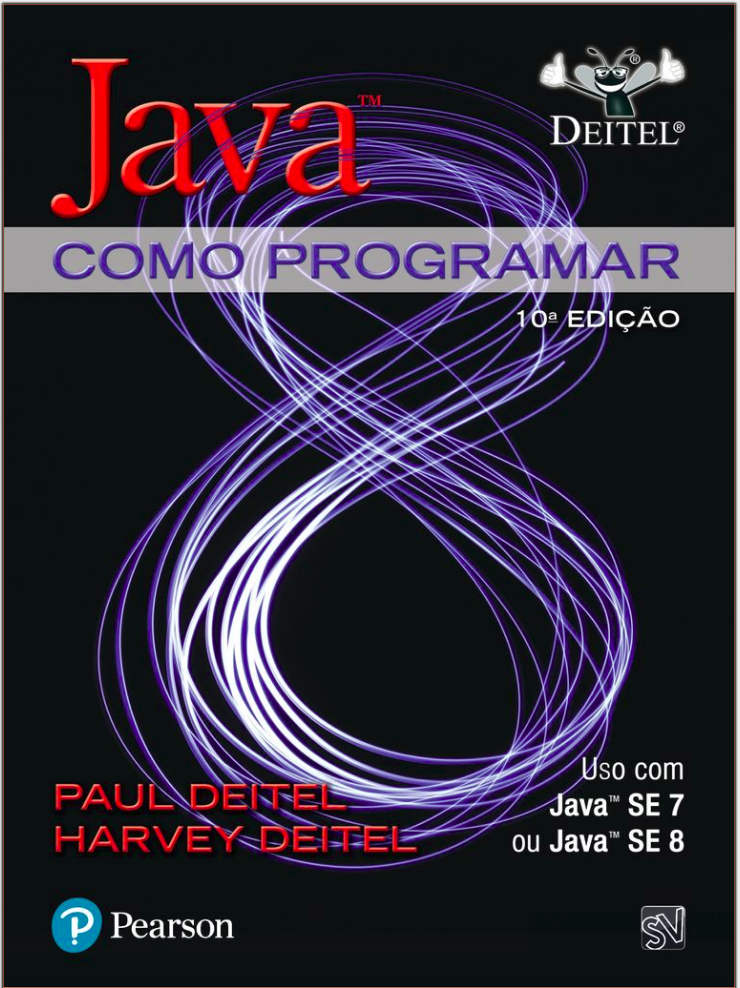
\includegraphics[height=0.6\paperheight]{fig/aula1/deitel2017java.png} 
	\end{column}
	\end{columns}
	%\textcolor{red}{DISPONÍVEL NA BIBLIOTECA VIRTUAL}
\end{frame}}

 %----------------------------------------------------------------------------
 
 \mode<presentation>{\begin{frame}{Referências}%[allowframebreaks]
 \small
 \begin{center}
 	\bibliographystyle{apalike}
	 \bibliography{ref_aula_progI}
 \end{center}
 \end{frame}}

\begin{figure}[!ht] \fbox{\includeslide[width=\textwidth]{slide:z}} \end{figure}
Text for notes goes here. 
\begin{itemize}
  \item List 1. 
  \item List 2. 
\end{itemize}


%%%%%%%%%%%%%%%%%% END MATTER %%%%%%%%%%%%%%%%%%
\end{document}